\documentclass[a4paper, fontsize=8pt, landscape, DIV=1]{scrartcl}
\usepackage{lastpage}
% Include general settings and customized commands
%
% General packages and settings
% ===========================================================================
% Author:			Silvano Cortesi (cortesis@student.ethz.ch)
% Version:			1.2
% Last changed:		03.01.2018
%
% ---------------------------------------------------------------------------




\usepackage[german]{babel} %choose your language \usepackage[german]{babel}
%\usepackage[T1]{fontenc}
\usepackage[utf8]{inputenc}
\usepackage{fancyhdr}
%\usepackage{lastpage}
%\usepackage{lmodern}
\usepackage{enumerate}
%\usepackage{float} % for positioning of figures
\usepackage[landscape, margin=1cm]{geometry}
\usepackage[dvipsnames]{xcolor}
\usepackage{pdfpages}


%% Math %%
\usepackage{amscd}
\usepackage{blindtext}
\usepackage{enumitem}
\usepackage{multicol}
\usepackage{parskip}
\usepackage{empheq}
\usepackage{amsmath}
\usepackage{amsfonts}
\usepackage{amssymb}
\usepackage{amsthm}
%\usepackage{dsfont}
%\usepackage{esint} % provides \oiint
\usepackage{mathrsfs}
%\usepackage{trfsigns}
%\numberwithin{equation}{subsection}
%\usepackage{numprint}
\usepackage{commath}

%% Graphics & Charts %%
\usepackage{graphicx}
%\usepackage{pdfpages}
%\usepackage{booktabs}
%\usepackage{array}
%\usepackage{paralist}
%\usepackage{framed}
%\usepackage{trfsigns}
\usepackage{tikz}
%\usepackage[lofdepth,lotdepth]{subfig}
%\usepackage{tikz}  %Graphen zeichnen
%\usetikzlibrary{decorations.pathmorphing}
%\usetikzlibrary{arrows.meta,arrows}
%\usepackage{pgfplots}
%% General Settings %%
%\setlength{\parindent}{0px}
%\setkomafont{captionlabel}{\normalfont\bfseries}
\usepackage{caption}

%\pagestyle{fancy}
%\lfoot{\tiny \today}
%\rfoot{\thepage\  / \pageref{LastPage}}
%\cfoot{}
%\renewcommand{\footrulewidth}{0.4pt}

%% provides command \uline{} for underlining words
%\usepackage{ulem}

%% colour headings
%\usepackage{color}
%\definecolor{bluen}{cmyk}{1,0.5,0,0}
%\definecolor{bloodorange}{cmyk}{0,.92,1,.2}
%\addtokomafont{section}{\color{bloodorange}}
%\addtokomafont{subsection}{\color{bloodorange}}
%\addtokomafont{subsubsection}{\color{bloodorange}}
%\addtokomafont{paragraph}{\small\color{bloodorange}}
%\addtokomafont{subparagraph}{\small\color{bloodorange}}

%% Signs & Special Formating %%
%\usepackage{ulem} %normalem: \emph{Text} is italic again.
%\usepackage{multicol,multirow}
%\usepackage{tabularx}
%\usepackage{stackrel}
%\usepackage{makeidx}
%\usepackage{mparhack} % bessere margiale bei seitenumbruch

% make document compact
\usepackage[compact]{titlesec}
\titlespacing{\section}{0pt}{*0}{*0}
\titlespacing{\subsection}{0pt}{*0}{*0}
\titlespacing{\subsubsection}{0pt}{*0}{*0}

\parindent 0pt
\pagestyle{empty}
\setlength{\unitlength}{1cm}
\setlist{leftmargin = *}

%include also newer PDF
\pdfminorversion=6

% Set the color of your style
% Avaiable are: Apricot, Aquamarine, Bittersweet, Black, Blue, blue, BlueGreen, BlueViolet, BrickRed, Brown, BurntOrange, CadetBlue, CarnationPink, Cerulean, CornflowerBlue, Cyan, Dandelion, DarkOrchid, Emerald, ForestGreen, Fuchsia, Goldenrod, Gray, Green, GreenYellow, JungleGreen, Lavender, ... (more at: http://en.wikibooks.org/wiki/LaTeX/Colors)
\def\StyleColor{CarnationPink}

% No indentation in multiline captions
% From: https://latex.org/forum/viewtopic.php?t=3248
\setcapindent{0pt}

%
% General commands
% ===========================================================================
% Author:			Silvano Cortesi (cortesis@student.ethz.ch)
% Version:			1.2
% Last changed:		03.01.2018
%
% ---------------------------------------------------------------------------

%..ROEMISCHE_ZAHLEN
	\newcommand{\Roe}[1]{\uppercase\expandafter{\romannumeral #1 }}

%..ZAHLENMENGEN
	\newcommand{\N}{\mathbb{N}}
	\newcommand{\Z}{\mathbb{Z}}
	\newcommand{\Q}{\mathbb{Q}}
	\newcommand{\R}{\mathbb{R}}
	\newcommand{\real}{\R}
	\newcommand{\C}{\mathbb{C}}
	\newcommand{\complex}{\C}
	\newcommand{\0}{\mathbb{O}}
	\newcommand{\F}{\mathbb{F}}
	\newcommand{\K}{\mathbb{K}}
    \newcommand{\angstrom}{\textup{\AA}}
    
%..PFEILE
	\renewcommand{\leadsto}{\Longrightarrow}
	\newcommand{\leftrightleadsto}{\Longleftrightarrow}

%..VEKTOREN
	\newcommand{\Ul} {\underline}
	\newcommand{\vEx} {\vec{e}_x}
	\newcommand{\vEy} {\vec{e}_y}
	\newcommand{\vEz} {\vec{e}_z}
	\newcommand{\vEq} {\vec{e_1}}
	\newcommand{\vEw} {\vec{e_2}}
	\newcommand{\vEe} {\vec{e_3}}
	\newcommand{\transpose} {^{\text{T}}}
	\newcommand{\vect}[1]{\boldsymbol{#1}}
	
%..MATRIX
    \newcommand{\MATR}[1]{ \displaystyle \left( \begin{matrix} #1 \end{matrix} \right)}
    \newcommand{\MATRABS}[1]{ \displaystyle \left| \begin{matrix} #1 \end{matrix} \right|}


%..KOMPLEXE ZAHLEN
	\renewcommand{\Re}{\text{Re}\,}
	\renewcommand{\Im}{\text{Im}\,}

%..OPERATOREN
	\DeclareMathOperator{\grad}{grad}
	\renewcommand{\div}{\text{div}\,}
    \DeclareMathOperator{\rot}{rot}
    \DeclareMathOperator{\divg}{div}
    \DeclareMathOperator{\Tr}{Tr}
    \DeclareMathOperator{\const}{const}
	\DeclareMathOperator{\imag}{i}
	\newcommand{\Lapl}{\hbox{\footnotesize{$\Delta$}}}

%..DIFFERENTIALRECHNUNG
	\newcommand{\Dx} {\,\mathrm{d}}
	\newcommand{\abl}[1] {\frac{\mathrm{d}}{\mathrm{d}#1}}
	\newcommand{\Abl}[2] {\frac{\mathrm{d}#1}{\mathrm{d}#2}}
	\newcommand{\ablq}[1] {\frac{\mathrm{d^2}}{\mathrm{d}#1^2}}
	\newcommand{\Ablq}[2] {\frac{\mathrm{d^2}#1}{\mathrm{d}#2^2}}
	\newcommand{\pabl}[1] {\frac{\partial}{\partial#1}}
	\newcommand{\pablq}[1] {\frac{\partial^2}{\partial#1^2}}
	\newcommand{\Pabl}[2] {\frac{\partial#1}{\partial#2}}
	\newcommand{\Pablq}[2] {\frac{\partial^2#1}{\partial#2^2}}

%..INTEGRALRECHNUNG
	\newcommand{\dint}{\displaystyle{\int}}
	\newcommand{\intab}{\int^b_a}
	\newcommand{\intinf}{\int_{-\infty}^\infty}
	\newcommand{\dintab}{\displaystyle{\int^b_a}}
	\newcommand{\dintpi}{\displaystyle{\int^{\pi}_{-\pi}}}
	\newcommand{\dintzpi}{\displaystyle{\int^{2\pi}_{\mbox{-}2\pi}}}
	\newcommand{\dA}{\hspace{4pt}\mathrm{d}A}
	\newcommand{\dx}{\hspace{4pt}\mathrm{d}x}
	\newcommand{\dy}{\hspace{4pt}\mathrm{d}y}
	\newcommand{\dz}{\hspace{4pt}\mathrm{d}z}
	\newcommand{\dr}{\hspace{4pt}\mathrm{d}r}
	\newcommand{\ds}{\hspace{4pt}\mathrm{d}s}
	\newcommand{\dS}{\hspace{4pt}\mathrm{d}S}
	\newcommand{\dt}{\hspace{4pt}\mathrm{d}t}
	\newcommand{\dm}{\hspace{4pt}\mathrm{d}m}
	\newcommand{\dk}{\hspace{4pt}\mathrm{d}k}
	\newcommand{\dl}{\hspace{4pt}\mathrm{d}l}
	\newcommand{\du}{\hspace{4pt}\mathrm{d}u}
	\newcommand{\dv}{\hspace{4pt}\mathrm{d}v}
	\newcommand{\dV}{\hspace{4pt}\mathrm{d}V}
	\newcommand{\dphi}{\hspace{4pt}\mathrm{d}\varphi}
	\newcommand{\domega}{\hspace{4pt}\mathrm{d}\omega}
	\newcommand{\dvarsigma}{\hspace{4pt}\mathrm{d}\varsigma}
	\newcommand{\dtau}{\hspace{4pt}\mathrm{d}\tau}
	\newcommand{\dtheta}{\hspace{4pt}\mathrm{d}\vartheta}
	\newcommand{\dmu}{\hspace{4pt}\mathrm{d}\mu}
	\newcommand{\dxi}{\hspace{4pt}\mathrm{d}\xi}
	\newcommand{\deta}{\hspace{4pt}\mathrm{d}\eta}
	\newcommand{\dvecl}{\hspace{4pt}\mathrm{d}\vec{l}}
	\newcommand{\dvecS}{\hspace{4pt}\mathrm{d}\vec{S}}

%..LIMES
    \DeclareMathOperator{\limni}{\lim\limits_{n\to\infty}}
    \DeclareMathOperator{\limxi}{\lim\limits_{x\to\infty}}
    \DeclareMathOperator{\limho}{\lim\limits_{h\to0}}
    \newcommand{\limxai}[1]{\ensuremath{\lim\limits_{x\to #1}}}

%..SUMMEN
    \DeclareMathOperator{\sumni}{\sum_{n=0}^{\infty}}
    \newcommand{\sumnia}[1]{\ensuremath{\sum_{n=#1}^{\infty}}}


%..PARTIELLE ABLEITUNG
    \DeclareMathOperator{\partf}{\dfrac{\partial f}{\partial x}}
    \newcommand{\partfo}[1]{\ensuremath{\dfrac{\partial f}{\partial #1}}}
    \newcommand{\parto}[1]{\ensuremath{\dfrac{\partial }{\partial #1}}}
    \newcommand{\partt}[2]{\ensuremath{\dfrac{\partial^2 }{\partial #1\partial #2}}}
    \newcommand{\partq}[1]{\ensuremath{\dfrac{\partial^2 }{\partial #1^2}}}


%..ENUMERATION
    \newenvironment{abc}{\begin{enumerate}[(a)]}{\end{enumerate}}
    \newenvironment{cabc}{\begin{compactenum}[(a)]}{\end{compactenum}}
    \newenvironment{romanenum}{\begin{enumerate}[i.]}{\end{enumerate}}
    \newenvironment{cromanenum}{\begin{compactenum}[i.]}{\end{compactenum}}

%..FUNCTIONS
    \DeclareMathOperator{\arsinh}{arsinh}
    \DeclareMathOperator{\arcosh}{arcosh}
    \DeclareMathOperator{\artanh}{artanh}
    \DeclareMathOperator{\arcoth}{arcoth}
    \DeclareMathOperator{\arccot}{arccot}
    \DeclareMathOperator{\Arg}{Arg}
    \DeclareMathOperator{\Log}{Log}
    \newcommand{\dis}[1]{\hspace{#1cm}}
    \newcommand{\abs}[1]{\ensuremath{\left\vert#1\right\vert}}
    \newcommand{\attention}{\raisebox{-1pt}{{\makebox[1.6em][c]{\makebox[0pt][c]{\raisebox{.13em}{\small!}}\makebox[0pt][c]{\color{red}\Large$\bigtriangleup$}}}}}
    \DeclareMathOperator{\meq}{\stackrel{!}{=}}
    
    
% section color box
\setkomafont{section}{\mysection}
\newcommand{\mysection}[1]{%
    \Large\sffamily\bfseries%
    \setlength{\fboxsep}{0cm}%already boxed
    \colorbox{\StyleColor!40}{%
        \begin{minipage}{\linewidth}%
            \vspace*{2pt}%Space before
            #1
            \vspace*{-1pt}%Space after
        \end{minipage}%
    }}

%subsection color box
\setkomafont{subsection}{\mysubsection}
\newcommand{\mysubsection}[1]{%
    \normalsize \sffamily\bfseries%
    \setlength{\fboxsep}{0cm}%already boxed
    \colorbox{\StyleColor!20}{%
        \begin{minipage}{\linewidth}%
            \vspace*{2pt}%Space before
             #1
            \vspace*{-1pt}%Space after
        \end{minipage}%
    }}

% highlighter
\newcommand{\hilight}[1]{\colorbox{\StyleColor}{#1}}

% equation box        
\newcommand{\eqbox}[1]{\setlength{\fboxrule}{1mm}\fcolorbox{\StyleColor}{white}{\hspace{0.5em}$\displaystyle#1$\hspace{0.5em}}}

%center equationbox
\newcommand{\ceqbox}[1]{\vspace*{4pt} \begin{center}\eqbox{#1}\end{center}\vspace*{4pt}}
%change page style for header
\pagestyle{fancy}
\footskip 6.7pt
\rhead{Felix Crazzolara}
\lhead{Reinforcement learning}
\chead{\thepage}

\title{Reinforcement learning}
\author{Felix Crazzolara}

\date{\today}
\begin{document}

\setcounter{secnumdepth}{2} %no enumeration of sections

\begin{multicols*}{3}

\maketitle 

\section{Stochastic processes\cite{Papoulis1965ProbabilityRV}}
$x[n]$ is called a \textit{discrete-state} process if its values are countable. Otherwise, it is a \textit{continuous-state} process.

\section{Dymamic programming}
Dynamic programming (DP) is an algorithmic technique for solving an optimization problem by breaking it down into simpler subproblems and utilizing the fact that the optimal solution to the overall problem depends upon the optimal solution to its subproblems.

\section{Policy gradient methods}
\subsection{Basics}
\textbf{The goal of reinforcement learning}\\[3pt]
\begin{align*}
\text{Infinite horizon:}&\quad\theta^*\triangleq\arg\max_{\theta}\mathbb{E}_{(s,a)\sim p_{\theta}(s,a)}[r(s,a)] \\[3pt]
\text{Finite horizon:}&\quad\theta^*\triangleq\arg\max_{\theta}\sum\limits_{t=1}^{T}\mathbb{E}_{(s_t,a_t)\sim p_{\theta}(s_t,a_t)}[r(s_t,a_t)]
\end{align*}

\textbf{The policy gradient (Finite horizon)}\\[3pt]
\begin{align*}
\nabla_{\theta}J(\theta)&=\nabla_{\theta}\mathbb{E}_{\tau\sim p_{\theta}(\tau)}[\sum\limits_{t=1}^{T}r(s_t,a_t)]=\int\nabla_{\theta}p_{\theta}(\tau)r(\tau)\dif\tau\\
&=\mathbb{E}_{\tau\sim p_{\theta}(\tau)}[\nabla_{\theta}\log p_{\theta}(\tau)r(\tau)] \\
&=\mathbb{E}_{\tau\sim p_{\theta}(\tau)}[\left(\sum\limits_{t=1}^{T}\nabla_{\theta}\log\pi_{\theta}(a_t|s_t)\right)\left(\sum\limits_{t=1}^{T}r(s_t,a_t)\right)]
\end{align*}
Note that the Markov property is not used here!

\textbf{The policy gradient (Finite horizon with discount)}
\begin{align*}
\nabla_{\theta}J(\theta)&=\nabla_{\theta}\mathbb{E}_{\tau\sim p_{\theta}(\tau)}[\sum\limits_{t=1}^{T}\gamma^{t-1}r(s_t,a_t)] \\
&=\mathbb{E}_{\tau\sim p_{\theta}(\tau)}[\left(\sum\limits_{t=1}^{T}\nabla_{\theta}\log\pi_{\theta}(a_t|s_t)\right)\left(\sum\limits_{t=1}^{T}\gamma^{t-1}r(s_t,a_t)\right)]
\end{align*}

\textbf{Causality (Finite horizon)}\\[3pt]
\begin{align*}
\nabla_{\theta}J(\theta)&=\sum\limits_{t=1}^{T}\mathbb{E}_{\substack{s_{1:t}\\a_{1:t}}}\left[\nabla_{\theta}\log\pi_{\theta}(a_t|s_t)\mathbb{E}_{\substack{s_{t+1:\infty}\\a_{t+1:\infty}}}\left[\sum\limits_{t'=1}^{T}r(s_{t'},a_{t'})\bigg\rvert s_{1:t},a_{1:t}\right]\right] \\
&=(*)
\end{align*}
With
\begin{equation*}
\mathbb{E}_{a_t|s_t}[\nabla_{\theta}\log\pi_{\theta}(a_t|s_t)]=\int\pi_\theta(a_t|s_t)\nabla_{\theta}\log\pi_{\theta}(a_t|s_t)\dif a_t=0,
\end{equation*}
it follows that
\begin{align*}
(*)&=\sum\limits_{t=1}^{T}\mathbb{E}_{\substack{s_{1:t}\\a_{1:t}}}\left[\nabla_{\theta}\log\pi_{\theta}(a_t|s_t)\mathbb{E}_{\substack{s_{t+1:\infty}\\a_{t+1:\infty}}}\left[\sum\limits_{t'=t}^{T}r(s_{t'},a_{t'})\bigg\rvert s_{1:t},a_{1:t}\right]\right] \\
&=\mathbb{E}_{\substack{s_{1:\infty}\\a_{1:\infty}}}\left[\sum\limits_{t=1}^{T}\nabla_{\theta}\log\pi_{\theta}(a_t|s_t)\left(\sum\limits_{t'=t}^{T}r(s_{t'},a_{t'})\right)\right]
\end{align*}

\textbf{Causality (Finite horizon with discount)}\\[3pt]
Similarly as before it holds that:
\begin{align*}
\nabla_{\theta}J(\theta)=\mathbb{E}_{\substack{s_{1:\infty}\\a_{1:\infty}}}\left[\sum\limits_{t=1}^{T}\nabla_{\theta}\log\pi_{\theta}(a_t|s_t)\left(\sum\limits_{t'=t}^{T}\gamma^{t'-1}r(s_{t'},a_{t'})\right)\right]
\end{align*}

\textbf{The off-policy policy gradient}\\[3pt]
\begin{align*}
\nabla_{\theta'}J(\theta')=\mathbb{E}_{\tau\sim p_{\theta}(\tau)}\Bigg[\sum\limits_{t=1}^{T}\nabla_{\theta'}\log\pi_{\theta'}(a_t|s_t)\left(\prod\limits_{t'=1}^{t}\frac{\pi_{\theta'}(a_{t'}|s_{t'})}{\pi_{\theta}(a_{t'}|s_{t'}}\right) \\
\left(\sum\limits_{t'=t}^{T}r(s_{t'},a_{t'})\left(\prod\limits_{t''=t}^{t'}\frac{\pi_{\theta'}(a_{t''}|s_{t''})}{\pi_{\theta}(a_{t''}|s_{t''}}\right)\right)\Bigg]
\end{align*}

\section{Papers}
\subsection{Introduction to Stochastic Dynamic Programming (1983)}
Consider a countable state set $\mathcal{S}$ and a finite action set $\mathcal{A}$. The states are are labelled by nonnegative integers and the transition probabilities are given by $P_{ij}(a)$ for $a\in\mathcal{A}$. Furthermore, upon choosing an action, a reward $|R(i,a)|<B$ is credited to the agent. The value function is defined as
\begin{equation*}
V_{\pi}(i)=\mathbb{E}_{\pi}\left[\sum\limits_{n=0}^{\infty}R(X_n,a_n)\alpha^n|X_0=i\right].
\end{equation*}
Let $V(i)=\sup_{\pi}V_{\pi}(i)$. A policy $\pi^*$ is said to be $\alpha$-optimal if $V_{\pi^*}(i)=V(i)$ for all $i\ge 0$. the optimal value function is satisfies an optimality equation:\\[3pt]
\textit{Theorem 2.1 (The Optimality Equation):} 
\begin{equation*}
V(i)=\max_a[R(i,a)+\alpha\sum_jP_{ij}(a)V(j)],\quad i\ge 0.
\end{equation*}
Finally, the next theorem establishes the existance of an optimal policy:\\[3pt]
\textit{Theorem 2.2:} Let $f$ be a mapping $f:\mathcal{S}\rightarrow\mathcal{A}$ which satisfies
\begin{small}
\begin{equation*}
R(i,f(i))+\alpha\sum_jP_{ij}(f(i))V(j)=\max_a[R(i,a)+\alpha\sum_jP_{ij}(a)V(j)],\quad i\ge 0.
\end{equation*}
\end{small}
Then $V_f(i)=V(i)$ for all $i\ge 0$, and hence $f$ is $\alpha$-optimal.

\subsection{Learning Without State-Estimation in Partially Observable Markovian Decision Processes}
\textit{Points out a few very interesting issues that can arise when applying RL methods to POMDPs.}
\begin{minipage}{0.6\columnwidth}
Hello \ref{fig:POMPD}
\end{minipage}
\begin{minipage}{0.4\columnwidth}
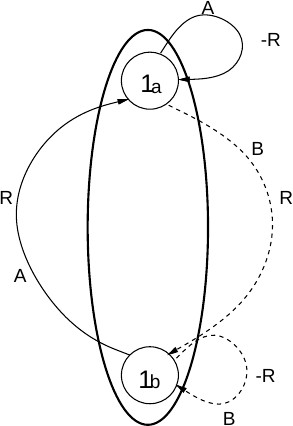
\includegraphics[width=\textwidth]{img/POMDP.jpg}
\label{fig:POMDP}
\captionof{figure}{POMDP with two states (1a\&1b), two actions (A\&B), but only one possible observation.}
\end{minipage}
\textit{Issue 1:} Any policy will incur a cost of $R$ per step, whereas the optimal behavior results in a reward of $R$ per step.
\textit{Issue 2:} The optimal policy for the POMDP is non-stationary.

\subsection{An Analysis of Temporal-Difference Learning with Function Approximation}
\textit{Assumption 1:} 1) The Markov chain $i_t$ is irreducible and aperiodic. Furthermore, there is a unique distribution $\pi$ that satisfies $\pi'P=\pi'$ with $\pi(i)>0$ for all $i$; here, $\pi$ is a finite of infinite vector, depending on the cardinality of $S$. Let $E_0[\cdot]$ stand for expectation with respect to this distribution.\\
2) Transition costs $g(i_t,i_{t+1})$ satisfy $E_0[g^2(i_t,i_{t+1})]<\infty$
\textit{Assumption 2:} 1) the matrix $\Phi$ has full column rank; that is, the basis functions $\{\phi_k|k=1,\ldots,K\}$ are linearly independent.\\
2) For every $k$, the basis function $\phi_k$ satisfies $E_0[\phi_k^2(i_t)]<\infty$.
\textit{Assumption 3:} There exists a function $f:S\rightarrow\mathbb{R}_+$ satisfying the following requirements:\\
1) For all $i_0$ and $m\ge0$
\begin{equation*}
\sum\limits_{\tau=0}^{\infty}||E[\phi(i_{\tau})\phi'(i_{\tau+m})|i_0]-E_0[\phi(i_t)\phi'(i_{t+m})]||\le f(i_0)
\end{equation*}
and
\begin{equation*}
\sum\limits_{\tau=0}^{\infty}||E[\phi(i_{\tau})g(i_{\tau+m},i_{\tau+m+1})|i_0]-E_0[\phi(i_t)g(i_{t+m},i_{t+m+1})]||\le f(i_0).
\end{equation*}
2) For any $q>1$, there exists a constant $\mu_q$ such that for all $i_0,t$ $E[f^q(i_t)|i_0]\le\mu_q f^q(i_0)$.
\textit{Assumption 4:}
The step sizes $\gamma_t$ are positive, nonincreasing, and predetermined. Furthermore, they satisfy $\sum\limits_{t=0}^{\infty}\gamma_t=\infty$ and $\sum\limits_{t=0}^{\infty}\gamma_t^2<\infty$.\\[5pt]
\textit{Theorem 1:} Under assumption 1-4, the following hold:\\
1) The cost-to-go function $J^*$ is in $L_2(S,D)$.\\
2) For any $\lambda\in[0,1]$, the TD($\lambda$) algorithm with linear function approximators converges with probability one.\\
3) The limit of convergence $r^*$ is the unique solution of the equation $\Pi T^{(\lambda)}(\Phi r^*)=\Phi r^*$.\\
4) Furthermore, $r^*$ satisfies
\begin{equation*}
||\Phi r^*-J^*||_D\le\frac{1-\lambda\alpha}{1-\alpha}|\Pi J^*-J^*|_D.
\end{equation*}

\subsection{Policy Gradient Methods for Reinforcement Learning with Function Approximation}
\textit{Establishes the policy gradient theorem and shows convergence of policy gradient algorithm for arbitrary policy classes.}\\[5pt]

\section{Tipps and tricks}
\subsection{Value function normalization}
Consider a reward function $R:\mathcal{S}\times\mathcal{A}\rightarrow[-R,R]$. If we define the normalized value function as $V_{\pi}^n(s)\triangleq(1-\gamma)V_{\pi}(s)$, where $V_{\pi}(s)\triangleq\mathbb{E}_{\substack{s_{0:\infty}\\a_{0:\infty}}}[\sum\limits_{t=0}^{\infty}\gamma^t\mathcal{R}(s_t,a_t)]$ is the usual value function and $\gamma\in(0,1)$ is the discount factor, then we are guarantueed that $V_{\pi}^n(s)\in[-R,R]$.

\bibliographystyle{plain}
\bibliography{references.bib}


\end{multicols*}


\setcounter{secnumdepth}{2}
\end{document}
